%\documentclass[preprint,showpacs,preprintnumbers,superscriptaddress,prb,floatfix,aps]{revtex4-1}
\documentclass[twocolumn,showpacs,preprintnumbers,superscriptaddress,prb,floatfix,aps,10pt]{revtex4-1}

\usepackage{amsmath,amssymb}
\usepackage{graphicx,textcomp}
\usepackage{physics} % bra-ket
\usepackage{braket}  % over-write bra-ket
\usepackage{epstopdf}
\usepackage{subfigure}
\usepackage{xfrac} % nice frac
\usepackage{multirow} % multirow table

\usepackage[version=3]{mhchem}
\usepackage{siunitx}
\sisetup{
  separate-uncertainty,
  output-open-uncertainty=[
}


\usepackage{xcolor}
\definecolor{abm}{RGB}{190,220,170}
\usepackage{todonotes}
\presetkeys%
    {todonotes}%
    {inline,backgroundcolor=abm}{}
%
\newcommand{\abmei}[1]{\textcolor{orange}{ \bf [Antonio: #1] }}
% \renewcommand{\vec}[1]{\ensuremath{\mathbf{#1}}}
\newcommand*{\ham}{\hat{H}}
\newcommand*{\class}{\mathcal{C}}
\newcommand*{\wignerD}{\mathbb{D}(R)}
\newcommand*{\wignerDl}{D^{(l)}(R)}
\newcommand*{\id}{\mathcal{E}}
\newcommand*{\zeromat}{0}
\newcommand*{\bloch}{\ket{\vec{k}, i\alpha}}
\newcommand*{\lowdin}{\ket{\vec{r}, i\alpha}}
\newcommand*{\x}{\times}
\newcommand*{\bondvec}{\vec{r}_{ij}}
\newcommand{\seitz}[2]{\{#1|#2\}}

\begin{document}
\pagenumbering{arabic}

\title{VN ARPES}

\author{A. B. Mei}
\affiliation{Department of Materials Science and the Materials Research Laboratory
University of Illinois, 104 South Goodwin, Urbana, IL 61801}

\author{L. Hultman}
\affiliation{Department of Physics, Chemistry and Biology (IFM), Link\"oping University, SE-581 83, Link\"oping, Sweden.}

\author{I. Petrov}
\affiliation{Department of Materials Science and the Materials Research Laboratory
University of Illinois, 104 South Goodwin, Urbana, IL 61801}
\affiliation{Department of Physics, Chemistry and Biology (IFM), Link\"oping University, SE-581 83, Link\"oping, Sweden.}

\author{J. E. Greene}
\affiliation{Department of Materials Science and the Materials Research Laboratory
University of Illinois, 104 South Goodwin, Urbana, IL 61801}
\affiliation{Department of Physics, Chemistry and Biology (IFM), Link\"oping University, SE-581 83, Link\"oping, Sweden.}

\begin{abstract}

This highly-efficient basis is able to accurately reproduce both electronic band dispersion determined by ARPES and ab-initio density functional theory simulations with a minimal set of fourteen empirical fitting parameters.
\end{abstract}

\maketitle

The electronic band dispersion and Fermi surface of VN is modeled using an emperical minimal-basis orthogonal tight-binding model. Energy-momentum dispersion relations $E(\vec{k})$ are obtained by solving the secular equation
% CARDONA p 88 + HESS p 36
\begin{equation}
\label{eq:secular}
\left| \ham^{\alpha\beta}_{ij}(\vec{k}) - E(\vec{k})\delta_{\alpha\beta}\delta_{ij} \right| = 0
\end{equation}
%
associated with the time-independent Schrodinger equation $\hat{H} \ket{\psi} = E \ket{\psi}$. $\delta$ are Kronecker deltas and $|\cdot |$ denotes matrix determinant. The eigenfunctions $\ket{\psi}$ of the Hamiltonian are linear combinations of periodic Bloch states $\bloch$ with expansion coefficients
$c_{i\alpha} = \braket{\vec{k},i\alpha | \psi}$:
% CARDONA p 88
\begin{align}
\ket{\psi}  &= \sum_{i\alpha} c_{i\alpha} \bloch
\end{align}
%
The Bloch states are, in turn, defined as the Fourier transform of L\"{o}wdin atomic-like states $\lowdin$:
% KITTEL p 246
\begin{equation}
\ket{\vec{k}} = \frac{1}{\sqrt{N}} \sum_i e^{i\vec{r}_i\cdot\vec{k}} \ket{\vec{r}, i\alpha}, 
\quad
\alpha \equiv (l,m).
\end{equation}
%
$\vec{k}$ are wave vectors. $\vec{r}_i$ specifies the coordinate of primitive atom $i$ on which orbital $\ket{i\alpha}$ is located. $l$ and $m$ are azimuthal and magnetic quantum number. N is the number of atoms in the crystal.

Matrix elements between different $\ket{\vec{k}}$ states vanish due to translational symmetry. 
% KITTEL p 247
\begin{equation}
\label{eq:ham}
\ham^{\alpha\beta}_{ij}(\vec{k}) 
= \frac{1}{N} \sum_{ij} H^{\alpha\beta}_{ij}(\vec{r}) e^{-i\vec{r}_{ij} \cdot \vec{k} } 
= \sum_j H^{\alpha\beta}_{ij}(\vec{r}) e^{-i\vec{r}_{ij} \cdot \vec{k}}
\end{equation}
%
in which
%
\begin{align}
\ham^{\alpha\beta}_{ij}(\vec{r}) &\equiv \bra{\vec{r},i\alpha} \ham\ket{\vec{r},j\beta} \\
\ham^{\alpha\beta}_{ij}(\vec{k}) &\equiv \bra{\vec{k},i\alpha} \ham\ket{\vec{k},j\beta}
\end{align}
%
are real-space and Fourier-transformed Hamiltonian matrix elements describing interactions between orbitals $\alpha$ and $\beta$ centered on primitive atom $i$ and neighbor $j$. $\bondvec = \vec{r}_i - \vec{r}_j$ represents the bond connecting sites $i$ and $j$. 

The B1 NaCl-structure lattice consists of two interpenetrating cation and anion face-centered cubic sublattices offset with respect to each other by half a primitive cell. Each cation (anion) has six equivalent first neighbor anions (cations) at $\bondvec = [0 0 \frac{1}{2}]$ and twelve second neighbor cations (anions) at $\bondvec = [0 \frac{1}{2} \frac{1}{2}]$. Explicitly describing interactions to second neighbors using a minimal orthogonal basis with cation-centered $d$ and anion-centered $p$ orbitals engenders the eight-dimensional Hilbert space:
\begin{align}
\label{eq:hilbert}
\psi &= \bigoplus_{i\alpha} \hat{c}_{i\alpha}^\dag \\
&= \left[ 
  \hat{c}^\dag_{\textrm{V} d \bar{2}},
  \hat{c}^\dag_{\textrm{V} d \bar{1}},
  \hat{c}^\dag_{\textrm{V} d  0},
  \hat{c}^\dag_{\textrm{V} d  1},
  \hat{c}^\dag_{\textrm{N} d  2},
  \hat{c}^\dag_{\textrm{N} p \bar{1}},
  \hat{c}^\dag_{\textrm{N} p  0},
  \hat{c}^\dag_{\textrm{N} p  1}
\right].
\end{align}
%
in which the ladder operators $c^\dag_{i\alpha}$ create electrons on orbitals $\ket{i\alpha}$. %For clarity, site indices $i$ are omitted in Eq. \ref{eq:hilbert} since $d$ and $p$ are exclusive to V and N sites in the minimal basis.

Evaluating the summation in Eq. \ref{eq:ham} to second neighbor yields 83 possibly different matrix elements. The tight-binding Hamiltonian, with the summation of neighbors $j$ shown explicitly, is
%
% \begin{widetext}
\begin{equation}
\label{eq:ham_explicit}
\ham(\vec{k}) = 
\begin{bmatrix}
\ham_{\textrm{V}0}^{dd}(\vec{k}) + \ham_{\textrm{V}2}^{dd}(\vec{k}) & -\ham_{\textrm{V}1}^{pd}(\vec{k}) \\
\ham_{\textrm{V}1}^{pd}(\vec{k})^{\dagger} & \ham_{\textrm{N}0}^{pp}(\vec{k}) + \ham_{\textrm{N}2}^{pp}(\vec{k}) \\
\end{bmatrix}
\end{equation}
% \end{widetext}
$\ham_{ij}^{ll'}$ are $(2l+1) \times (2l'+1)$ submatrices describing coupling of states with different magnetic quantum numbers. 

 Crystallographic and orbital symmetries are utilized to identify an irreducible set of fourteen symmetry-adapted matrix elements. 
 
 
 
 
The transformation of state vectors, necessary for establishing symmetry relations between matrix elements,  
%
\begin{equation}
\wignerD \ket{i\alpha} \rightarrow \ket{j\beta}
\end{equation}
%
is realized through $\wignerD$, which corresponds to the representation of symmetry $R$ engendered by the basis:
%
\begin{align}
\wignerD = \bigoplus_l \wignerDl
\end{align}
%
Wigner functions
\begin{equation}
\wignerDl = e^{- \hat{n} \cdot \hat{L} /\hbar}
\end{equation}
are $(2l+1)$-dimensional square matrix which parameterize proper rotations. % Lax p 43 Eq 2.5.18
Improper rotations are obtained by premultiplying $(-1)^l$ with the scalar inversion operator. \cite{sharma_general_1979,el-batanouny_symmetry_2008} The direct sum is performed over azimuthal quantum numbers $l$ in the primitive cell. 
% Wooten p 604 bottom, under Eq. 14.164 



 
 
 
 
 
 
 Due to orbital parity, matrix elements transform as:
%
\begin{equation}
\label{eq:intrinsic}
v_{ij}^{\alpha\beta} = (-1)^{l+l'}v_{ji}^{\beta\alpha}
\end{equation}
%
under interchange of orbitals positions. $l$ and $l'$ are azimuthal quantum number associated with orbitals $\alpha$ and $\beta$. 


%


Together, these symmetries enforce additional relationships between matrix elements:
%
\begin{equation}
\label{eq:stab}
v_{ij}^{\alpha\beta} = \sum_{\mu\nu} v_{ij}^{\mu\nu} \left[\wignerD\right]_{\mu\alpha} \left[\wignerD\right]_{\nu\beta}.
\end{equation}
%
$\left[\phantom{.}\cdot\phantom{.}\right]_{\mu\alpha}$ selects element $\mu\alpha$ of the enclosed matrix. $\wignerD$ are symmetry representations engendered by the tight binding basis and describe the coupling of states with different magnetic quantum numbers. Formulations for $\wignerD$ are provided in Appendix 





The crystallographic point group of the NaCl lattice is $O_h$(m$\bar{3}$m). $O_h$(m$\bar{3}$m) contains forty-eight symmetry operations. Twenty-four are proper rotations belonging to the chiral octahedral subgroup $O$(432) and may be further subdivided among five conjugacy classes\footnote{Classes $\class_i$ are mutually distinct sets containing symmetries $R_i$ and $R_j$ related by conjugation with $R_k$ an arbitrary group element: $R_kR_iR_k^{-1}=R_j$} --  $\id$, $3c_4^2$, $6c_2$, $8c_3$, and $6c_4$ -- which correspond to the identity, two-fold rotations about $\left<001\right>$, two-fold rotations around $\left<011\right>$, three-fold rotations about $\left<111\right>$, and four-fold rotations around $\left<001\right>$. The additional twenty-four symmetries are improper rotations formed by compounding $O$ symmetries with the inversion operator $i$ and also display a similar structure consisting of five conjugacy classes. $i$, $3\sigma_2$, $6\sigma_2$, $8\sigma_6$, and $6\sigma_4$ are associated with inversion, reflection across $\{001\}$, reflection across $\{011\}$, three-fold roto-inversions around $\left<111\right>$, and four-fold roto-inversions about $\left<001\right>$. The $O_h$ group has two generators, \footnote{The generating basis of a group is a minimal set of elements which is capable of producing all elements in the group when multiplied together.} $c_4$ and $\sigma_6$ which, uniquely specify all crystallographic symmetric relations among tight-binding matrix elements.

On-site tight-binding matrix elements are subject to the full point group symmetry of the NaCl lattice. In order to determine the irreducible set of symmetry-adapted matrix elements, the point group is analyzed using character representation theory. Irreducible characters are determined using the Burnside algorithm (see Appendix \ref{appendix:chartab}) and the results are summarized in Table \ref{table:chartab}. Also shown are the irreducible characters of $p$ and $d$ tesseral harmonics, the direct sum $p \oplus d$, and of the outer products $p \otimes p$, $p \otimes d$, and $d \otimes d$. 

In descending from the full three-dimensional rotational group $SO(3)$ to the crystallographic point group $O_h$, the three-fold degeneracy of $p$ orbitals is preserved as $T_{1u}$ a triply-degenerate irreducible representation. As a result, elements between $p$ states transform as the outer product $T_{1u} \otimes T_{1u} = [A_{1g} \oplus E_g \oplus T_{2g}] \oplus \{T_{1g}\}$ with the terms in square and curly brackets corresponding to symmetric and antisymmetric components. In the $p$ orbital basis, $T_{1g}$ and $T_{2g}$ are three-dimensional matrices with nonzero elements at off-diagonal positions; $E_g$ is a traceless matrix with nonzero elements at diagonal positions; and $A_{1g}$ is the identity matrix. \footnote{Representative basis functions for $T_{1g}$, $T_{2g}$, $E_g$, and $A_{1g}$ are $\ket{x}\bra{y} - \ket{y}\bra{x}$, $\ket{x}\bra{y} + \ket{y}\bra{x}$, $\ket{x}\bra{x} + e^{i2\pi/3}\ket{y}\bra{y} + e^{-i2\pi/3}\ket{z}\bra{z}$, and $\ket{x}\bra{x} + \ket{y}\bra{y} + \ket{z}\bra{z}$.} The \emph{single} occurrence of $A_{1g}$ in the decomposition of $T_{1u} \otimes T_{1u}$ signifies the existence a \emph{single} symmetry-adapted tight-binding matrix element, which is identified as $\epsilon_p$ the energy of the three-fold-degenerate $p$ states. The sub-Hamitonian describing on-site $p$ interactions is thus:
%
\begin{equation}
\label{eq:0pp}
\ham_0^{pp} =
\begin{bmatrix}
\epsilon_{p} & 0 & 0 \\
0 & \epsilon_{p} & 0 \\
0 & 0 & \epsilon_{p} \\
\end{bmatrix}
\end{equation}
%

\begin{table}
\caption{\label{table:chartab} $O_h$ representation characters}
\begin{ruledtabular}
\begin{tabular*}{10cm}{llrrrrrrrrrr}
\multicolumn{2}{c}{$O_h$}         &$\id$&3$c_4^2$& 6$c_2$ & 8$c_3$ & 6$c_4$ &  $i$ & 3$\sigma_2$ & 6$\sigma_2$ & 8$\sigma_6$ & 6$\sigma_4$ \\  
\hline
$A_{1g}$        & $\Gamma_{1}  $  &  1  &     1  &     1  &     1  &     1  &   1  &          1  &          1  &          1  &          1  \\         %  irrep =  1 
$A_{2g}$        & $\Gamma_{2}  $  &  1  &     1  &    -1  &     1  &    -1  &   1  &          1  &         -1  &          1  &         -1  \\         %  irrep =  2 
$E_g   $        & $\Gamma_{12} $  &  2  &     2  &     0  &    -1  &     0  &   2  &          2  &          0  &         -1  &          0  \\         %  irrep =  3 
$T_{1g}$        & $\Gamma_{15} $  &  3  &    -1  &    -1  &     0  &     1  &   3  &         -1  &         -1  &          0  &          1  \\         %  irrep =  5 
$T_{2g}$        & $\Gamma_{25} $  &  3  &    -1  &     1  &     0  &    -1  &   3  &         -1  &          1  &          0  &         -1  \\         %  irrep =  4 
$A_{1u}$        & $\Gamma_{1} '$  &  1  &     1  &     1  &     1  &     1  &  -1  &         -1  &         -1  &         -1  &         -1  \\         %  irrep =  7 
$A_{2u}$        & $\Gamma_{2} '$  &  1  &     1  &    -1  &     1  &    -1  &  -1  &         -1  &          1  &         -1  &          1  \\         %  irrep =  6 
$E_u   $        & $\Gamma_{12}'$  &  2  &     2  &     0  &    -1  &     0  &  -2  &         -2  &          0  &          1  &          0  \\         %  irrep =  8 
$T_{1u}$        & $\Gamma_{15}'$  &  3  &    -1  &    -1  &     0  &     1  &  -3  &          1  &          1  &          0  &         -1  \\         %  irrep =  9 
$T_{2u}$        & $\Gamma_{25}'$  &  3  &    -1  &     1  &     0  &    -1  &  -3  &          1  &         -1  &          0  &          1  \\ \hline \hline %  irrep = 10 
\multicolumn{2}{c}{$C_{4v}$}      &$\id$& $c_4^2$&        &        & 2$c_4$ &      & 2$\sigma_v$ &  $\sigma_d$ &             &             \\ 
\hline
$A_1$           & $\Delta_{1}  $  &  1  &     1  &     .  &     .  &     1  &   .  &          1  &          1  &          .  &          .  \\         %  irrep =  1
$A_2$           & $\Delta_{1}' $  &  1  &     1  &     .  &     .  &     1  &   .  &         -1  &         -1  &          .  &          .  \\         %  irrep =  4
$B_1$           & $\Delta_{2}  $  &  1  &     1  &     .  &     .  &    -1  &   .  &          1  &         -1  &          .  &          .  \\         %  irrep =  3
$B_2$           & $\Delta_{2}' $  &  1  &     1  &     .  &     .  &    -1  &   .  &         -1  &          1  &          .  &          .  \\         %  irrep =  2
$E$             & $\Delta_{5}  $  &  2  &    -2  &     .  &     .  &     0  &   .  &          0  &          0  &          .  &          .  \\ \hline \hline %  irrep =  5
\multicolumn{2}{c}{$C_{2v}$}      &$\id$&        &  $c_2$ &        &        &      &  $\sigma_v$ & $\sigma_d$  &             &             \\
\hline
$A_{1}$         & $\Sigma_{1}  $  &  1  &     .  &     1  &     .  &     .  &   .  &          1  &          1  &          .  &          .  \\
$A_{2}$         & $\Sigma_{2}  $  &  1  &     .  &     1  &     .  &     .  &   .  &         -1  &         -1  &          .  &          .  \\
$B_{1}$         & $\Sigma_{3}  $  &  1  &     .  &    -1  &     .  &     .  &   .  &         -1  &          1  &          .  &          .  \\
$B_{2}$         & $\Sigma_{4}  $  &  1  &     .  &    -1  &     .  &     .  &   .  &          1  &         -1  &          .  &          .  \\ \hline \hline
\multicolumn{2}{c}{$C_{3v}$}      &$\id$&        &        & 2$c_3$ &        &      &             & 3$\sigma_v$ &             &             \\
\hline
$A_{1}$         & $\Lambda_{1} $  &  1  &     .  &     .  &     1  &     .  &   .  &          .  &          1  &          .  &          .  \\
$A_{2}$         & $\Lambda_{2} $  &  1  &     .  &     .  &     1  &     .  &   .  &          .  &         -1  &          .  &          .  \\
$E$             & $\Lambda_{3} $  &  2  &     .  &     .  &    -1  &     .  &   .  &          .  &          0  &          .  &          .  \\ \hline \hline
\multicolumn{2}{c}{$p$          } &  3  &     -1 &    -1  &     0  &     1  &  -3  &          1  &          1  &          0  &         -1  \\
\hline
\multicolumn{2}{c}{$d$          } &  5  &      1 &     1  &    -1  &    -1  &   5  &          1  &          1  &         -1  &         -1  \\
\multicolumn{2}{c}{$p \oplus  d$} &  8  &      0 &     0  &    -1  &     0  &   2  &          2  &          2  &         -1  &         -2  \\
\multicolumn{2}{c}{$p \otimes p$} &  9  &      1 &     1  &     0  &     1  &   9  &          1  &          1  &          0  &          1  \\
\multicolumn{2}{c}{$p \otimes d$} & 15  &     -1 &    -1  &     0  &    -1  & -15  &          1  &          1  &          0  &          1  \\
\multicolumn{2}{c}{$d \otimes d$} & 25  &      1 &     1  &     1  &     1  &  25  &          1  &          1  &          1  &          1  \\
\end{tabular*}
\end{ruledtabular}
\end{table}
%
The lower symmetry of $O_h$ versus $SO(3)$ lifts the five-fold degeneracy on V 3$d$ orbitals, producing a two-dimensional $E_g$ and a three-dimensional $T_{2g}$ irreducible representation. The outer product $E_g \otimes E_g$ decomposes into $[A_{1g} \oplus E_g] \oplus \{A_{2g}\}$ and $T_{2g} \otimes T_{2g}$ reduces to $[A_{1g} \oplus E_{g} \oplus T_{2g}] \oplus \{T_{1g}\}$. The presence of the identity representation in both products indicates the existence of two independent matrix elements, corresponding to $\epsilon_e$ and $\epsilon_t$ the energies of V 3$d$ $E_g$ and $T_{2g}$ states. The cross-product $T_{2g} \otimes E_g = T_{1g} \oplus T_{2g}$ does not contain $A_{1g}$ in its decomposition and therefore vanishes. As a result, matrix elements for same-shell V $d$ self-interactions are:

%   1 -> A_1g
%   2 -> A_2g
%   3 -> E_g 
%   4 -> T_2g
%   5 -> T_1g
%   6 -> A_1u
%   7 -> A_2u
%   8 -> E_u 
%   9 -> T_2u
%  10 -> T_1u

\begin{equation}
\label{eq:0dd}
\mathbb{V}_0^{dd} =
\begin{bmatrix}
 \epsilon_{e} & 0 & 0 & 0 & 0 \\
 0 & \epsilon_{e} & 0 & 0 & 0 \\
 0 & 0 & \epsilon_{t} & 0 & 0 \\
 0 & 0 & 0 & \epsilon_{t} & 0 \\
 0 & 0 & 0 & 0 & \epsilon_{t} \\
\end{bmatrix}
\end{equation}

Eqs. \ref{eq:0pp} and \ref{eq:0dd} reveal that same-shell interactions yield dispersionless energy integrals, with $\epsilon_p$, $\epsilon_e$, and $\epsilon_t$ representing electronic band energies in the continuum limit ($\vec{k} \rightarrow \Gamma$).

% introduce subgroup and stabilizer group here.

Crystallographic symmetries either stabilize bond vectors $\bondvec$ or rotate them onto their symmetric equivalents. The set of rotations and reflections which leave $\bondvec$ invariant represent the bond stabilizer group. First neighbor bonds $\bondvec = [00\frac{1}{2}]$ are stabilized by symmetries belonging to $C_{4v}$ (4mm), a subgroup of $O_h$. These include the identity $\id \seitz{1}{0}$ as well as a two-fold $c_{4}^2$ and two four-fold $c_{4}$ rotations around $\bondvec$: $\seitz{2_{001}}{0}$, $\seitz{2_{001}}{0}$, $\seitz{4^-_{001}}{0}$, and $\seitz{4^+_{001}}{0}$. In addition, there are four mirror planes, of which two are vertical-reflection planes $\sigma_v$, $\seitz{m_{010}}{0}$ and $\seitz{m_{100}}{0}$, and two are diagonal reflection planes $\sigma_d$, $\seitz{m_{\frac{1}{2}\bar{\frac{1}{2}}0}}{0}$ and $\seitz{m_{\frac{1}{2}\frac{1}{2}0}}{0}$. $\bondvec$ resides at the intersection of mirror plans. The generators of the group are $c_4$ and $\sigma_v$. 

\abmei{NEED TRANSITION HERE}
Subduced $O_h$ representations are computed as described in Appendix \abmei{XX} and the results are summarized in Table \ref{table:subduction}. $d$ states factor as $E_g \rightarrow A_1 \oplus B_1$ and $T_{2g} \rightarrow B_2 \oplus E$, $p$ states reduce as $T_{1u} \rightarrow A_1 \oplus E$. The only two nonvanishing hopping elements occur between identity-containing products $A_1 \otimes A_1 = A_1$ and $E \otimes E = [ A_1 \oplus B_1 \oplus B_2 ] \oplus \{ A_2 \} $. From the commutator relationship $[\mathbb{V},\wignerD] = 0$ for group generators $R$, the two independent matrix elements are identified as $( 1, 0)$ and $( 0, 1)$. In addition, two symmetry relations are obtained 
\begin{align}
     (+2,-1) &= \phantom{\sqrt{3}} (+1, 0) \\
     (-2,+1) &=          \sqrt{3}  ( 0,+1)
\end{align}
The remaining eleven parameters are null. Summing over equivalent first neighbors yields the sub-Hamiltonian matrix:
%
\begin{table}
\caption{\label{table:subduction} $O_h$ subductions}
\begin{ruledtabular}
\begin{tabular*}{10cm}{llll}
$O_h$    & $C_{4v}$         & $C_{2v}$                              &   $C_{3v}$            \\ \hline
$A_{1g}$ & $A_1$            & $A_{1}$                               &   $A_1$               \\ 
$A_{2g}$ & $B_1$            & $B_{1}$                               &   $A_2$               \\ 
$E_g   $ & $A_1 \oplus B_1$ & $A_{1} \oplus B_{1}$                  &   $E$                 \\ 
$T_{1g}$ & $A_2 \oplus E$   & $A_{2} \oplus B_{1} \oplus B_{2}$     &   $A_2 \oplus E$      \\ 
$T_{2g}$ & $B_2 \oplus E$   & $A_{1} \oplus A_{2} \oplus B_{2}$     &   $A_1 \oplus E$      \\ 
$A_{1u}$ & $A_2$            & $A_{2}$                               &   $A_2$               \\ 
$A_{2u}$ & $B_2$            & $B_{2}$                               &   $A_1$               \\ 
$E_u   $ & $A_2 \oplus B_2$ & $A_{2} \oplus B_{2}$                  &   $E$                 \\ 
$T_{1u}$ & $A_1 \oplus E$   & $A_{1} \oplus B_{1} \oplus B_{2}$     &   $A_1 \oplus E$      \\ 
$T_{2u}$ & $B_1 \oplus E$   & $A_{1} \oplus A_{2} \oplus B_{1}$     &   $A_2 \oplus E$      \\ 
\end{tabular*}
\end{ruledtabular}
\end{table}
%
\begin{equation}
\mathbb{V}_1^{pd} =  2i
\begin{bmatrix}
-\sqrt{3} s_1 v_{ep} & 0            & \sqrt{3} s_3 v_{ep}  \\ % v5 = V(eg,p)
 s_1 v_{ep}          &-2 s_2 v_{ep} &  s_3 v_{ep}          \\ % v4 = V(t2g,p)
 s_2 v_{tp}          &  s_1 v_{tp}  & 0                    \\
0                    &  s_3 v_{tp}  &  s_2 v_{tp}          \\
 s_3 v_{tp}          & 0            &  s_1 v_{tp}          \\
\end{bmatrix}
\end{equation}
%
For concision, the following trigonometric abbreviations are employed: $c_i = \cos(\pi a k_i)$, $s_i = \sin(\pi a k_i)$, $s_{ij} = s_i s_j$ and $c_{ij} = c_i c_j$, in which $k_i = \vec{k}\cdot\hat{i}$ and $a = 0.4134$ nm, the experimentally-determined relaxed VN lattice parameter. The inclusion of off-site neighbor interactions associated with finite bond vectors (i.e., $\vec{r}_{ij} \neq 0$) introduces nontrivial Fourier components and contribute hoping elements that modulate band energies as a function of wave vector $\vec{k}$ throughout the Brillouin zone. 

% The $O_h$ point group has twelve $C_{2v}$ subgroups. Six belong to the intermediate subgroup of $C_{4v}$ and six are maximal subgroups of $O_h$.\cite{wadhawan_introduction_2000} The proper choice of subgroup affects the the subduction of $O_h$ irreducible representations onto the .

Second neighbor bonds $\bondvec = [0\frac{1}{2}\frac{1}{2}]$ are stabilized by subgroup $C_{2v}$ (2mm), consisting of four symmetries: identity $\id \seitz{1}{0}$, two-fold rotation $c_2 \seitz{ 2_{0\frac{1}{2}\frac{1}{2}} }{0}$, vertical-mirror plane $\sigma_v \seitz{m_{001}}{0}$, and diagonal mirror plane $\sigma_d \seitz{m_{0\frac{1}{2}\bar{\frac{1}{2}}}}{0}$. The two latter elements are group generators.




% [should already have introduced representations and irreps]
% CAPTION TO FIGURE?
$O_h$ exhibits ten irreducible representations $\Gamma^{(\mu)}$. These are labeled according to both Mulliken\footnote{In Mulliken notation, letters A,E,G, and H denote irreducible representations of dimensions one, two, three, and four. B is used in lieu of A for symmetries which are antisymmetric with respect to the principal axis (the axis of highest cyclical symmetry). Subscripts pairs $g$ and $u$, $1$ and $2$ as well as single and double primes are used to denote representations displaying even and odd parities with respect to inversion, horizontal two-fold rotations $c_2$, and horizontal reflections $\sigma_h$.} and BSW.


The group is non-Abelian with . The two group generators, $\sigma_6$ and $c_4$, fully define symmetry relations.
matrix element 


The three dimensional representations arise from non-commuting three-fold and six-fold symmetry elements. 




As required by translational symmetry, the crystallographic point groups exhibit integer characters.







$O_h$



All ten $O_h$ conjugacy classes produced by the outer product $O \otimes C_i$ are presented in the first row of Table \ref{table:chartab}.




\ref{appendix:wigner}.
%
Organizing the elements $v_{ij}^{\alpha\beta}$ in matrix form $\mathbb{V}$, Eq. \ref{eq:stab} is equivalent to
\begin{equation}
[\mathbb{V},\wignerD] = 0, 
\end{equation}
which indicates that stabilizer symmetries commute with $\mathbb{V}$ the matrix representation in the tight binding basis.






\begin{figure}
\label{fig:kappa_vs_t}
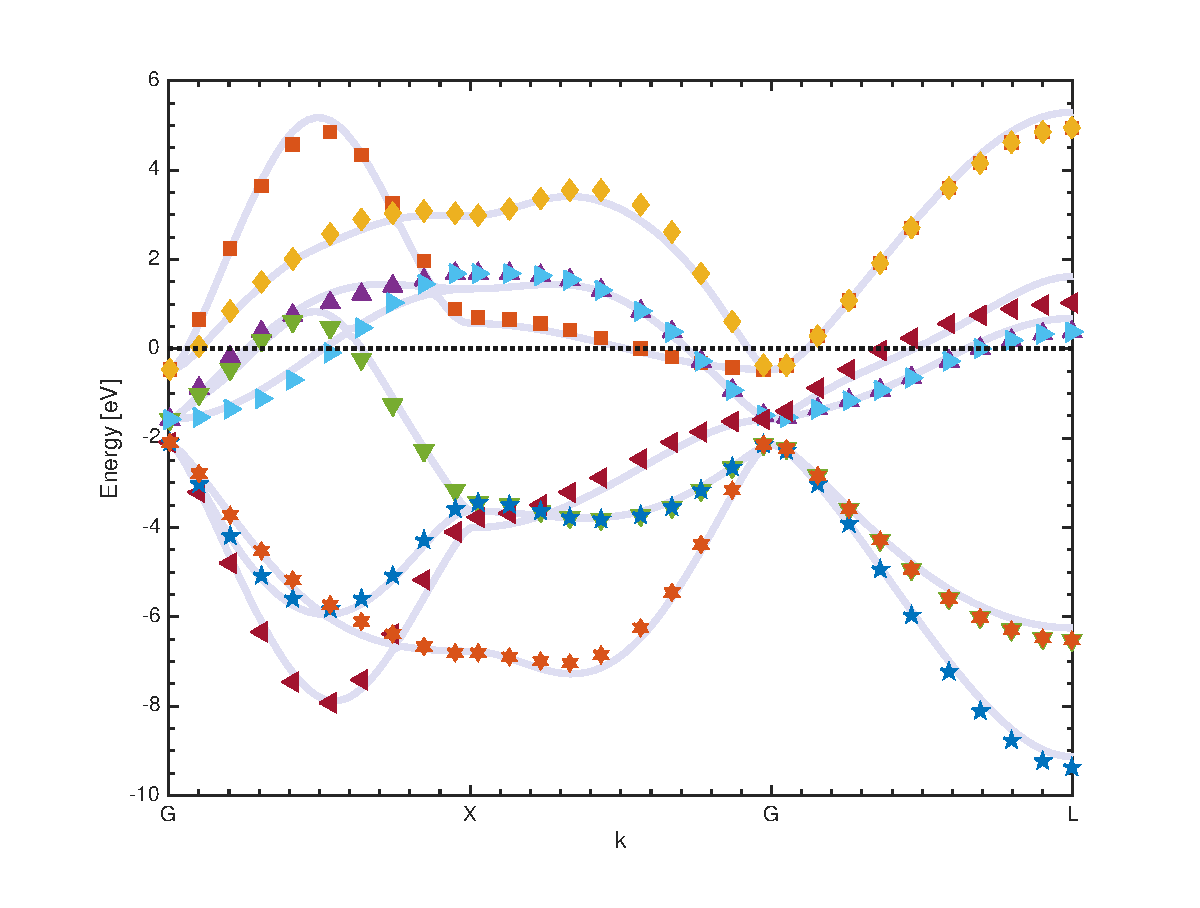
\includegraphics[width=0.5\textwidth]{band_structure.eps}
\caption{Bare electronic bands dispersion obtained from DFT GGA (solid lines) and orthogonal TB with optimized material parameters (symbols). } 
\end{figure}



\section{Acknowledgements}

\bibliography{library}

\clearpage

VN pd tb parameters

    1.2783
   -0.4859
   -3.9389
    1.0091
    1.0350
   -0.1245
   -0.2168
   -0.0825
   -0.5461
    0.0509
    0.1387
   -0.1257
    0.4381
    0.2954




\appendix

%
% WIGNER D MATRIX
%
\section{wigner D matrix} 
\label{appendix:wigner}

In terms of Tait-Bryan angles:
%
\footnote{
Conversion of $3\x3$ transformation matrices $R = R_x(\theta)R_y(\phi)R_z(\gamma)$ to Tait-Bryan angles $\theta$, $\phi$, and $\gamma$ representing rotations about $\hat{z}$, $\hat{y}$, and $\hat{x}$ axes is achieved via:
\begin{equation}
\theta = {\rm atan2}(R_{23},R_{33})
\end{equation}
\begin{equation}
\phi   =-{\rm atan2}(-R_{13},\sqrt{R_{11}^2+R_{12}^2})
\end{equation}
\begin{equation}
\begin{split}
\gamma =-{\rm atan2}(R_{31}\sin{\theta}-R_{21}\cos{\theta}, \\ 
       \quad         R_{22}\cos{\theta}-R_{32}\sin{\theta})
\end{split}
\end{equation}
${\rm atan2}$ is the four-quadrant arctangent function and $R_{ij}$ are the elements $ij$ of $R$. This formulation avoids gimbal lock.} 
%
\begin{equation}
\wignerDl = e^{-i\theta\hat{L}_x/\hbar} e^{-i\phi\hat{L}_y/\hbar} e^{-i\psi\hat{L}_z/\hbar}
\end{equation}
%
in which angular momentum operators:
%
\footnote{For numerical stability, the exponentiated operators are evaluated using the property: \abmei{XX} } \cite{shankar_fundamentals_2014}
%
\begin{align}
\label{eq:angular_momenta}
% x y z <- z x y
% Shankar p 327-328, Eq. 12.5.21a-b
% Wolfram p 85-87
\hat{L}_x & = \hbar (\hat{L}_{+}-\hat{L}_{-})/2i \\
\hat{L}_y & = \hbar m \delta_{l,l'}\delta_{m,m'} \\
\hat{L}_z & = \hbar (\hat{L}_{+}+\hat{L}_{-})/2
\end{align}
$\hat{L}_+$ and $\hat{L}_-$ are raising and lowering operators, with matrix elements:
\begin{equation}
\label{eq:raising_lowering_operator}
% Shankar p 327, Eq. 12.5.20
\hat{L}_{\pm} = \delta_{l,l'}\delta_{m\pm1,m'} \sqrt{(l\mp m)(l\pm m+1)},
\end{equation}









The conversion from spherical to cubic harmonics, $\ket{lm} \rightarrow \ket{\alpha}$, is achieved by conjugating $\wignerDl$ with:
\begin{equation}
\label{eq:cubic_harmonics}
Y_{lm} = 
\begin{cases}
\delta_{mm}                                      & \text{if } m = 0 \\
 i[(-1)^{m}\delta_{-mm'}-\delta_{ mm'}]/\sqrt{2} & \text{if } m > 0 \\
  [(-1)^{m}\delta_{ mm'}+\delta_{-mm'}]/\sqrt{2} & \text{if } m < 0
\end{cases}
\end{equation}




%
% TIGHT BINDING MODEL
%
\section{tight binding model}
\label{appendix:tb}













in which
\begin{widetext}
\begin{equation}
H_2^{dd} = 4
\begin{bmatrix}
 \tfrac{1}{\sqrt{3}} [c_{x} (c_{z}-2 c_{y})-2 c_{yz}] v_{6} & \multirow{2}{*}{$c_{y} (c_{z}-c_{x}) v_{6}$}    & \multirow{2}{*}{$-\sqrt{3} s_{xy} v_{8}$} & \multirow{2}{*}{$\sqrt{3} s_{yz} v_{8}$} & \multirow{2}{*}{$0$}               \\
             +\left[c_{yz}+c_{x} (c_{y}+c_{z})\right] v_{7} &                                                 &                                           &                                          &                                    \\
\multirow{2}{*}{.}                                          &     [c_{yz}+c_{x} (c_{y}+c_{z})] v_{7}          & \multirow{2}{*}{$-s_{xy} v_{8}$}          & \multirow{2}{*}{$-s_{yz} v_{8}$}         & \multirow{2}{*}{$2 s_{zx} v_{8}$}  \\ 
                                                            &                 -\sqrt{3} c_{zx} v_{6}          &                                           &                                          &                                    \\
\multirow{2}{*}{.}                                          & \multirow{2}{*}{.}                              &      (c_{x}+c_{y}) c_{z} v_{11}           & \multirow{2}{*}{$-s_{zx} v_{10}$}        & \multirow{2}{*}{$ s_{yz} v_{10}$}  \\    
                                                            &                                                 &                  +c_{xy} v_{9}            &                                          &                                    \\
\multirow{2}{*}{.}                                          & \multirow{2}{*}{.}                              & \multirow{2}{*}{.}                        &      c_{x} (c_{y}+c_{z}) v_{11}          & \multirow{2}{*}{$-s_{xy} v_{10}$}  \\
                                                            &                                                 &                                           &                  +c_{yz} v_{9}           &                                    \\
\multirow{2}{*}{.}                                          & \multirow{2}{*}{.}                              & \multirow{2}{*}{.}                        & \multirow{2}{*}{.}                       &      c_{y} (c_{x}+c_{z}) v_{11}    \\
                                                            &                                                 &                                           &                                          &                  +c_{zx} v_{9}     \\
\end{bmatrix}
\end{equation}
\end{widetext}


\begin{equation}
H^{pp}_2 =  4
\begin{bmatrix}
              c_{yz} v_{12} & \multirow{2}{*}{$-s_{xy} v_{13}$} & \multirow{2}{*}{$-s_{zx} v_{13}$}  \\
+c_{x} (c_{y}+c_{z}) v_{14} &                                   &                                    \\
\multirow{2}{*}{.}          &               c_{zx} v_{12}       & \multirow{2}{*}{$-s_{yz} v_{13}$}  \\
                            & +c_{y} (c_{z}+c_{x}) v_{14}       &                                    \\
\multirow{2}{*}{.}          & \multirow{2}{*}{.}                &          c_{xy} v_{12}             \\ 
                            &                                   &        +c_{z} (c_{x}+c_{y}) v_{14} \\
\end{bmatrix}
\end{equation}





%\section{Film growth and characterization}

\section{$O_h$}
\label{appendix:pg}
\section{Calculation of irreducible characters}
\label{appendix:chartab}
Characters $\chi_{i\mu}$ corresponding to irreducible representation $\Gamma_\mu$ and class $\class_i$ are determined using the Burnside algorithm.\cite{burnside_theory_2010,mckay_construction_1970,unger_computing_2006,schneider_dixons_1990,dixon_high_1967} In this approach, class products are decomposed into class sums:
\begin{equation}
\label{eq:class_coefficients}
\class_i \class_j = \sum_k h_{jk}^{(i)} \class_k
\end{equation}
with $h_{jk}^{(i)}$ being the frequency at which $\class_k$ appears in the multiplication of classes $\class_i$ and $\class_j$. The collection of class coefficient matrices $h^{(i)}$ are then simultaneously diagonalized using a matrix pencil approach, producing eigenvalues $\lambda_{i\mu}$ from which the dimensions of irreducible representations
\begin{equation}
\label{eq:irrep_dimension}
d_\mu = \sqrt{ \frac{|g|}{\sum_i \lambda_{i\mu} \lambda^{\dag}_{i\mu} / n_i }  }
\end{equation}
and their characters
\begin{equation}
\label{eq:irrep_characters}
\chi_{i\mu} = \frac{d_\mu \lambda_{i\mu}}{n_i}
\end{equation}
are computed. $n_i$ and $|g|$ are the number of elements in the class $i$ and the group. Elements in the same class have the same character.

Reduction coefficients $n_\mu$, defined as the number of times an irreducible representation $\Gamma^\mu$ appears in a reducible representation $\Gamma$:
\begin{equation}
\label{eq:irrep_decomposition}
\Gamma = \bigoplus_\alpha n_\alpha \Gamma_{i\alpha}
\end{equation}
are obtained from:
\begin{equation}
\label{eq:irrep_decomposition_coefficients}
% Wolfram p 20
n_\alpha = \frac{1}{|g|} \sum_i \chi\left(\Gamma_{i\alpha}\right)^\dag \chi\left(\Gamma_i\right)
\end{equation}
The sum is over classes $i$, with number of elements $h_i$, and characters corresponding to the $\alpha$ irreducible representation $\chi(\Gamma_i^\alpha)$.





%
%
%




\end{document}

